% !Mode:: "TeX:UTF-8"

\chapter{节点结构属性对社团演化影响因素的探究}
上一章介绍了动态复杂网络社团检测的相关研究以及城市风险计算的最新进展。上一章提到了社团演化对动态复杂网络社团检测的影响非常大,而目前的大部分方法都聚焦于动态复杂网络的每个时间快照上的社团检测效果而或多或少地忽略了社团演化的重要性。更进一步,本文认为节点的结构属性特别是局部结构对节点社团演化的影响是很大的,因为社团的演化行为是由节点的社团转移行为构成的,也就是说,节点的社团转移行为才是社团演化的驱动力量。因此针对节点的结构属性对节点社团转移的影响的探究是必要且重要的。这也是本章的研究重点,即对节点的结构属性对节点社团转移的影响的探究。本章首先介绍对探究节点结构属性对节点社团转移影响的方法,然后介绍使用的真实世界复杂网络数据集,随后介绍经过第一部分介绍的方法结合第二部分真实数据集分析后得到的结论。
\section{探究方法}

\begin{figure}[!htbp]
	\setlength{\abovecaptionskip}{0pt} 
	\setlength{\belowcaptionskip}{10pt} 
	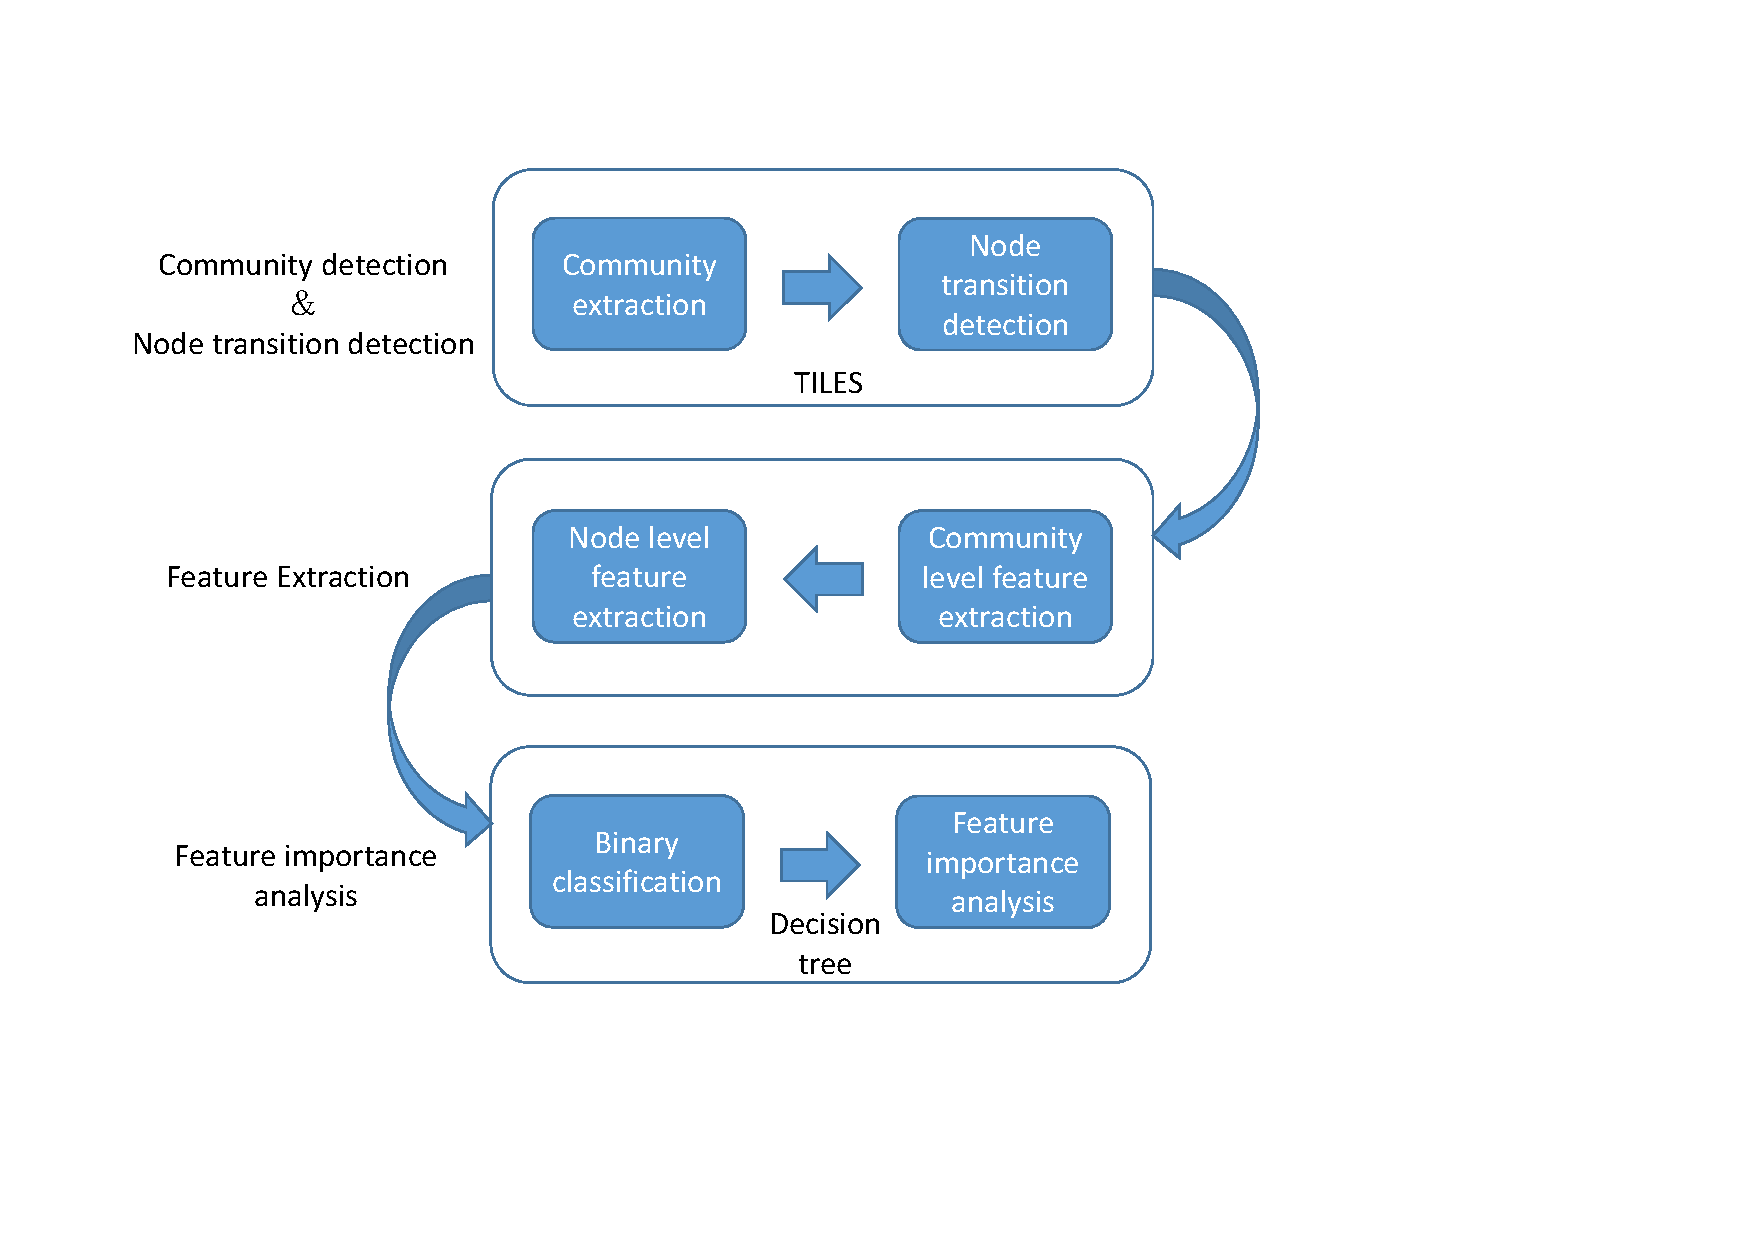
\includegraphics[width=.9\textwidth]{./figure/flowChart3.pdf}
	\caption{探究方法流程图}
	\label{fig.3.1}
\end{figure}

针对节店结构属性对节点社团转移影响的探究方法如图\ref{fig.3.1}所示,该方法共分为三步。
\begin{enumerate}
	\item 社团检测及节点转移检测,首先利用TILES\cite{rossetti2017tiles}对动态网络数据进行社团检测,同时TILES还会将复杂网络三元组数据进行时间片切分,即将$(源点,汇点,时间)$形式的数据处理为传统的动态网络时间片结构$W=\{W^1,W^2,...,W^T\}$,其中$T$为动态网络时间片的个数,而$W^t \in {0,1}^{N \times N}$为$t$时刻的网络邻接矩阵。我们假设所有该框架涉及到的网络均为无权图。随后我们将相邻的网络时间片组成相邻时间片组,并标注其中发生社团转移的节点与未发生社团转移的节点作为分类的节点社团转移标签。
	\item 节点结构特征提取,通过特征工程方法及以往论文的经验\cite{ilhan2016feature},本方法分别提取了五个社团级别结构特征及五个节点级别结构特征共十个结构特征。这些特征分别为:社团节点数、社团边数、社团内部边(即指向社团内部节点的边数)、社团外部边(即从社团内指出的边)、社团活性、社团的传导率、节点度、节点的平均邻居度、节点的接近中心性、节点的介数中心性。其具体描述见表\ref{fig.3.1}。通过相邻时间片组提取节点结构属性的方法见算法\ref{alg1}。
	\item 特征重要性分析,利用决策树对节点社团转移标签进行分类,将第二步提取的节点结构特征作为分类特征进行二分类。分类后,利用MDI计算每个特征在分类任务中的重要性,最终得到不同节点结构特征在节点发生社团转移情景中的重要性。
\end{enumerate}

在该框架的第一步中,框架利用了现有的社团检测框架TILES。TILES是现有的最高水准的基于进化聚类的社团检测算法,其利用标签传播方法检测动态网络中的社团,并在该进程中划分每个动态网络时间片。TILES检测的社团结构是重叠社团,即网络中每个节点可以在一个网络快照中属于多个社团,这给社团转移检测造成了一定难度,即如何界定节点发生社团转移行为。TILES认为重叠社团类似社交网络中的账号可以属于多个圈子,针对这种思路,本框架认为当一个节点在上一时间片转移到本时间片时,其社团归属集中有新社团出现时,则该社团发生了社团转移,因为一个人的精力是有限的,那么当这个人加入了新的社团时,其在原社团中投入的精力就会减小,这也是节点的一种社团转移。

在特征提取步骤中,本文认为节点所属社团也会对节点的转移行为造成影响,例如,在社交网络中,不同的圈子人员流动性是不一样的,或者如不同的组织人员流动性是不一样的。这些组织或群体的特征会影响群体内人员的转移意愿,因此本框架引入了部分社团级别的特征作为节点的结构特征的一部分。

在特征重要性分析中,本文选择了决策树来作为节点转移二分类的分类方法,因为决策树不同于深度神经网络,是白箱算法,因此每个特征的重要性都能通过决策树得到。本文使用Mean Decrease in Impurity(MDI)\cite{menze2009comparison}计算每个特征的重要性,DMI的定义如下:

\begin{equation}
\centering
\Delta i(s,r) = i(r)- p_L i(r_L) - p_R i(r_R)
\end{equation}

其中, $i(r)$ 是一些不纯度度量如gini index. $r$表示某个决策树节点,而$r_L$和$r_R$分别是 $r$的子节点。 $p_L = N_{r_L}/N_r$ 其中$N_r$是通过节点$r$的数据量。类似的$p_R=N_{r_R}/N_r$. 标准化后的$\Delta i(s,r)$可以给每个特征一个重要性度量,同时该计算指标非常高效,因此可以适用于大规模数据。

\begin{table}[!htbp]
	
	\centering
	\caption{notations and definitions}\label{tab.3.1}
	\resizebox{0.99\textwidth}{!}{
		\begin{tabular}{|l|p{70pt}|p{170pt}|l|}
			% \begin{tabular}{|l|l|l|l|}
			\hline
			Symbol&Feature & Description & Definition\\
			\hline
			$f1$&Community node number & Number of nodes within the community $l$ at time $t$. & $n_l^t$\\
			$f2$&Community edge number & Number of edges within the community $l$ at time $t$. & $e_l^t$\\
			$f3$&Intra community edges & Ratio of the total number of edges between the nodes inside the community($e_l^t(in)$) to the number of nodes in the community.& $\frac{e_l^t(in)}{n_l^t}$\\
			$f4$&Inter community edges & Ratio of the total number of edges of nodes connected outside the community($e_l^t(out)$) to the number of nodes in the community. & $\frac{e_l^t(out)}{n_l^t}$\\
			$f5$&Community activity & Ratio of the total number of connections made in the previous snapshot by the nodes of the community($a_l^t$) to the number of nodes in the community. & $\frac{a_l^t}{n_l^t}$\\
			$f6$&Community Conductance & Ratio of the number of edges in the community to the sum of degrees of the nodes in the community. & $\frac{e_l^t}{d_l^t}$\\
			$f7$&Node degree & Sum of links connected to node $i$ at time $t$. & $e_i^t$ \\
			$f8$&Node average neighbor degree & Average degree of node $i$'s neighbors, where $N(i)^t$ are the neighbors of node $i$ at time $t$ and $e_j^t$ is the degree of node $j$ which belongs to $N(i)^t$. & $\frac{1}{|N(i)^t|}\sum_{j\in N(i)^t}e_j^t$ \\
			$f9$&Node closeness centrality & Measuring a node $i$'s average path length to other nodes in community, where $C_{l,-i}^t$ is a set of all nodes in community $l$ except $i$ at time $t$ and $d(i,j)$ is the distance between node i and j.& $\sum_{j\in C_{l,-i}^t}\frac{C_l^t}{d(i,j)}$ \\
			$f10$&Node betweenness centrality & Measuring a node $i$'s importance in its community connectivity, where $\sigma_{jk}$ is the total number of shortest paths from node $j$ to node $k$ and $\sigma_{jk}(i)$ is the number of those paths that pass through $i$ & $\sum_{j,k \in C_{l,-i}^t}\frac{\sigma_{jk}(i)}{\sigma_{jk}}$\\
			\hline
		\end{tabular}
	}
\end{table}


\begin{algorithm}[!htbp]
	\caption{Feature extraction}
	\label{alg1}
	\algorithmicrequire \quad A sequence of undirected graphs $W = {W}^1,..{W}^T$ and the community assignment $\mathcal{C} = \mathcal{C}^1,...\mathcal{C}^T$\\
	\algorithmicensure \quad Nodes feature set $F$ and nodes label set $L$
	\begin{algorithmic}[1]
		\FOR{every graph ${W}^t$ where $t \neq T$}
		\FOR{every community $\mathcal{C}_l^t$ in $\mathcal{C}^t$ }
		\STATE Calculate community level features $F_c$
		\FOR{every node $i$ in community $\mathcal{C}_l^t$}
		\STATE Calculate node level features $F_n$
		\STATE Compose node $i$'s feature sequence $F = F_c + F_n$
		\IF{node $i$ changes its community in ${W}^{t+1}$}
		\STATE node $i$'s label $L_i$ = 1
		\ELSE
		\STATE node $i$'s label $L_i$ = 0
		\ENDIF
		\ENDFOR
		\ENDFOR
		\ENDFOR
	\end{algorithmic}
\end{algorithm}




\section{数据集}

本章所用数据集包括因特网数据、Facebook数据、手机信令数据即Wiki数据等共15个多类型网络公开复杂网络数据集,对于数据集的详细描述见表\ref{tab.3.2}。如图\ref{fig.3.2}所示,所有数据的节点度分布都服从power-law。




\begin{table}[!htbp]
	\centering
	\caption{data sets description}\label{tab.3.2}
	\resizebox{0.99\textwidth}{!}{
		\begin{tabular}{|p{70pt}|p{250pt}|p{40pt}|p{40pt}|}
			\hline
			Name & Description & $|\mathcal{V}|$ & $|\mathcal{E}|$\\
			\hline
			Internet & Internet\cite{mislove-2009-socialnetworksthesis} topology during $04/01/2004 -04/04/2005.$& $33936$ & $104824$\\
			Facebook & Facebook New Orleans networks\cite{viswanath-2009-activity} friends links during $06/08/2008-21/01/2009.$&$62306$& $905565$\\
			bitcoin & Who-trusts-whom network of people who trade using Bitcoin on Bitcoin OTC \cite{kumar2016edge} during $09/11/2010-19/01/2016.$ & $5881$ & $35592$\\
			Friend & Call logs of members of a young-family residential living community adjacent to a major research university in North America\cite{aharony2011social} during $10/07/2010-16/07/2011.$ & $130$ & $60518$\\
			fb-forum & The Facebook-like Forum Network\cite{nr} during $15/05/2004-24/10/2004.$ & $899$ & $33720$\\
			fb-messages & The Facebook-like Social Network\cite{nr} from an online community for students at University of California during $24/03/2004-22/10/2004.$ & $1897$ & $61734$\\
			ia-digg-reply & A reply network of the social news website Digg\cite{nr} during $29/10/2008-13/11/2008.$ & $30397$ & $87627$\\
			ia-facebook-wall-wosn-dir & The Facebook friendship graph\cite{nr} during $15/05/2004-24/10/2004.$ & $44668$ & $876993$\\
			ia-reality-call & The MIT Reality mining a small set of human call logs data\cite{nr} during $24/09/2004-07/01/2005. $& $6810$ & $52050$\\
			ia-slashdot-reply-dir & Reply network of technology website Slashdot\cite{nr} during $01/12/2005-31/08/2006.$ & $51097$ & $140778$\\
			ia-stackexch-user-marks-post & User answering question network of Stack Overflow\cite{nr} during $03/10/2008-25/11/2011.$ & $545196$ & $1302439$\\
			ia-yahoo-messages & The message network in yahoo\cite{nr} with time presented by  link sequences. & $99303$& $3179718$\\
			soc-epinions-trust-dir & Epinion who-trusts-whom network\cite{nr} with time presented by  link sequences. & $131828$ & $841373$\\
			soc-wiki-elec & Wikipedia adminship election data\cite{nr}during $14/09/2004-05/01/2008.$ & $8271$ & $107071$\\
			wiki& The Wikipedia links data \cite{mislove-2009-socialnetworksthesis} during $20/02/2001-06/12/2002.$ & $329623$ &$39953145$\\
			\hline
		\end{tabular}
	}
\end{table}


\begin{figure}[!htbp]
	\setlength{\abovecaptionskip}{0pt} 
	\setlength{\belowcaptionskip}{10pt} 
	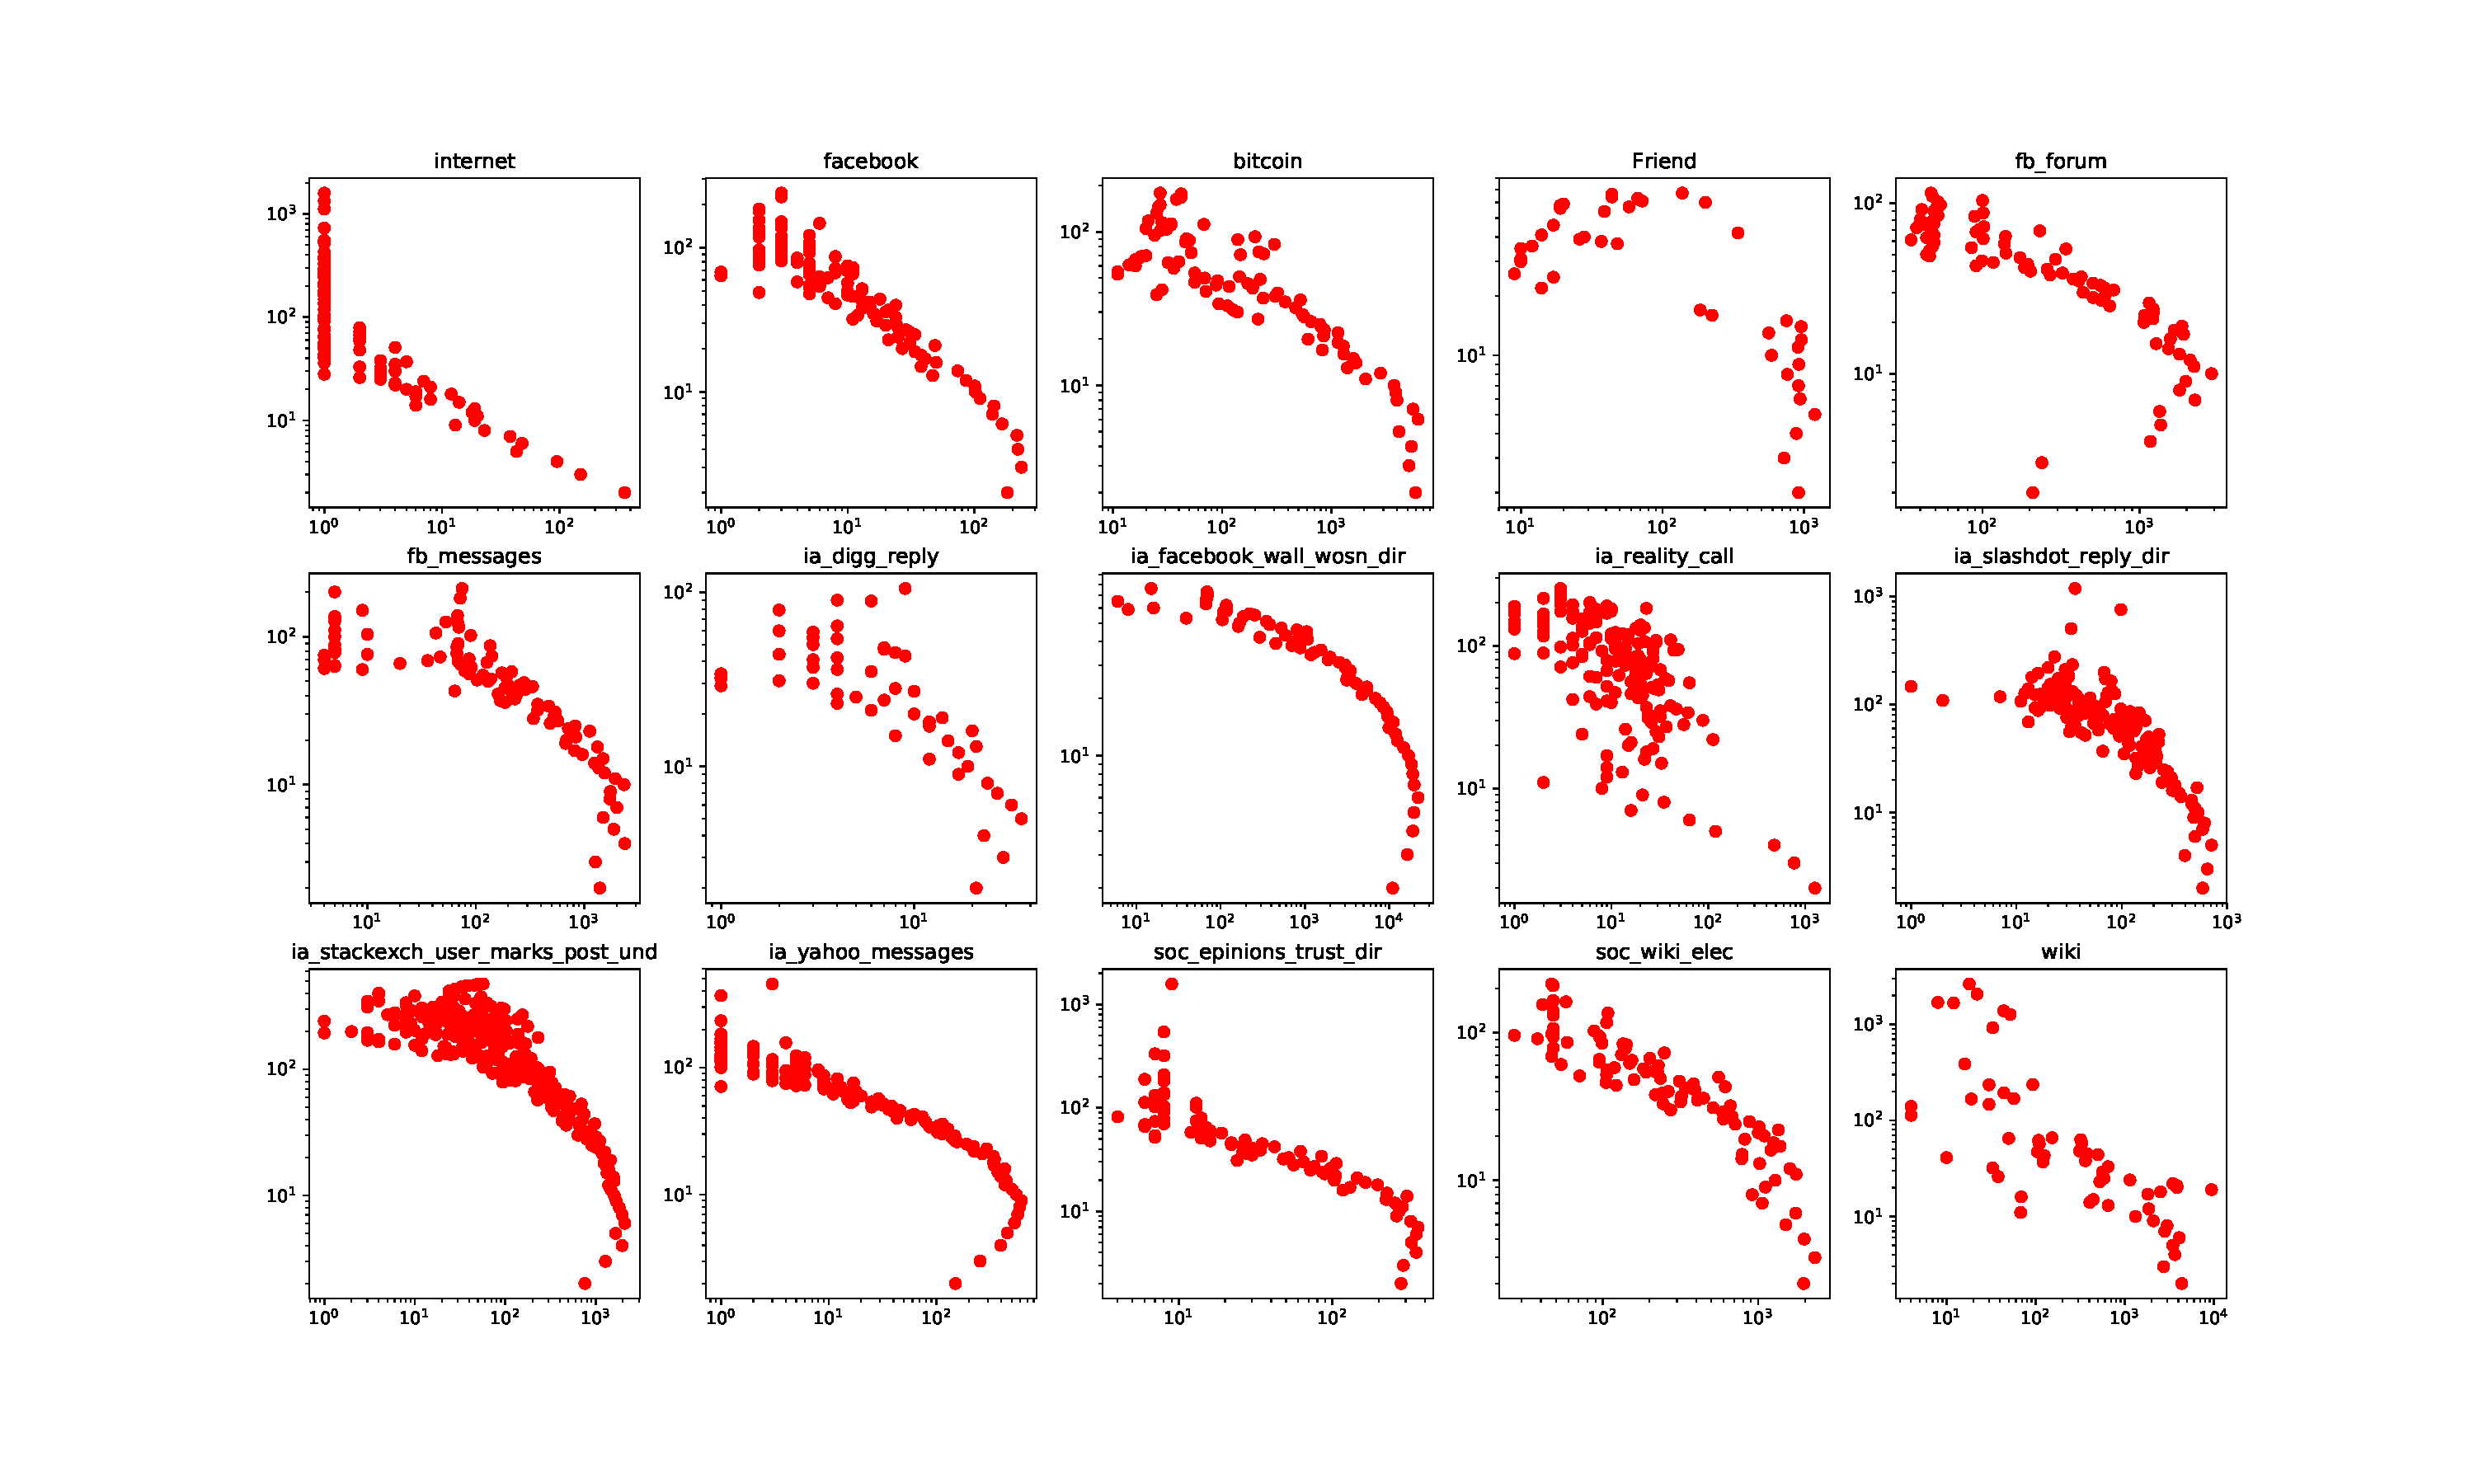
\includegraphics[width=.9\textwidth]{./figure/degrees.pdf}
	\caption{15个真实数据集的度分布可视化}
	\label{fig.3.2}
\end{figure}

\section{实验及验证}

\subsection{实验及结论}

按照上文所述的研究框架处理上述$15$个数据集,并计算其特征重要性。结果如热图\ref{fig.3.3}所示,横坐标表示节点的分类特征,即分类特征;纵坐标分别表示$15$个数据集,颜色代表特征在不同数据集中的分类任务中所占重要性。可以看到$f7$(节点的度)与$f8$(节点的平均邻居度)在所有特征分类中均占很大比重,尤其在$fb-forum$数据中,节点的平均邻居度在分类中所占比重超过了0.5;而$f5$(社团活跃度)在$ia-slashdot-reply-dir$数据中所占比重超过其他数据,该数据为技术网站Slashdot的回复网络,从这一点来看,\textbf{科技类网站的圈子活跃度}是影响其用户更换兴趣圈的主要因素;与此同时,在$internet$网络中,$f9$(节点的接近中心性)对其节点的社团转移影响最大,显而易见,在因特网中,连通性是其最至关重要的指标之一。虽然$f5,f9$均在某些数据集中显示出了对节点社团转移的重要影响力,但是其并不具有普遍性。反观$f7,f8$,其在所有数据集中对节点的社团转移均具有可观的影响力。因此我们得出结论,\textbf{节点的度以及节点的平均邻居度是影响节点发生社团转移的重要的结构特征}。


\begin{figure}[!htbp]
	\setlength{\abovecaptionskip}{0pt} 
	\setlength{\belowcaptionskip}{10pt} 
	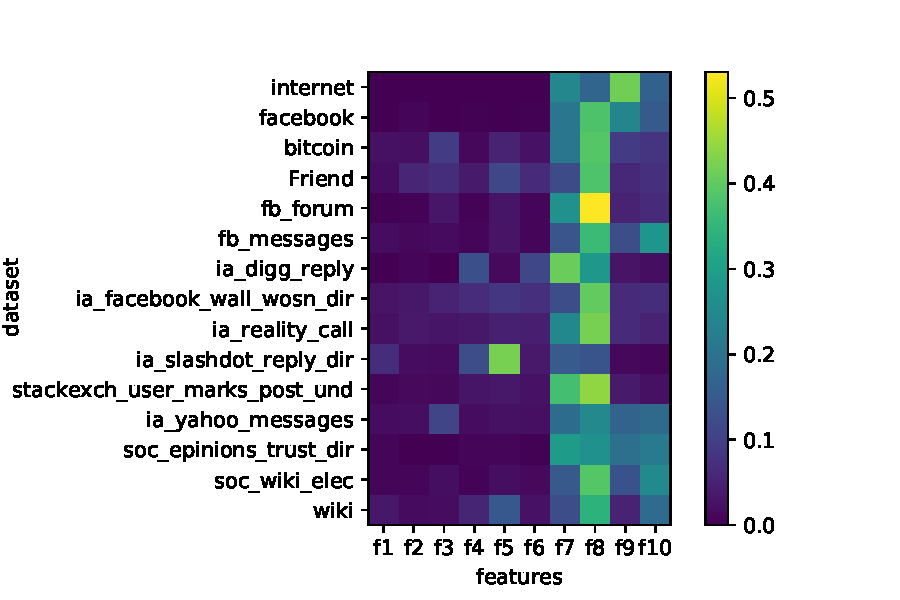
\includegraphics[width=.9\textwidth]{./figure/15cmp.pdf}
	\caption{15个数据集的特征重要性热图}
	\label{fig.3.3}
\end{figure}

为了探究节点的度以及节点的平均邻居度是以何种模式影响节点的社团转移的,本文分别统计了以上两个节点结构属性在$15$个数据集中的分布。如图\ref{fig.3.4}所示,该图展示了节点的度在十五个数据集中的分位图,每个子图中共有两列分位图,分别为发生转移的节点(横坐标为$1$)以及未发生转移的节点(横坐标为$0$)的度的分位统计图。从图中可以看到,在所有$15$个数据集中,发生社团转移的节点的度普遍比未发生转移的节点的度更高,即在一个网络中,节点的度越高,其越有可能转移其所在的社团。这也验证了社团检测中的大量度修正方法~\cite{wilson2016modeling,jin2015modeling}的正确性。而图\ref{fig.3.5}则展示了节点的平均邻居度在十五个数据集中的分位图,每个子图中共有两列分位图,分别为发生转移的节点(横坐标为$1$)以及未发生转移的节点(横坐标为$0$)的平均邻居度的分位统计图。可以看到节点的平均邻居度在不同数据集中的发生转移以及未发生转移节点中的值并不相同,这说明不同的节点平均邻居度确实在影响节点的社团转移行为,然而其模式在所有十五个数据集中并不统一。

\begin{figure}[!htbp]
	\setlength{\abovecaptionskip}{0pt} 
	\setlength{\belowcaptionskip}{10pt} 
	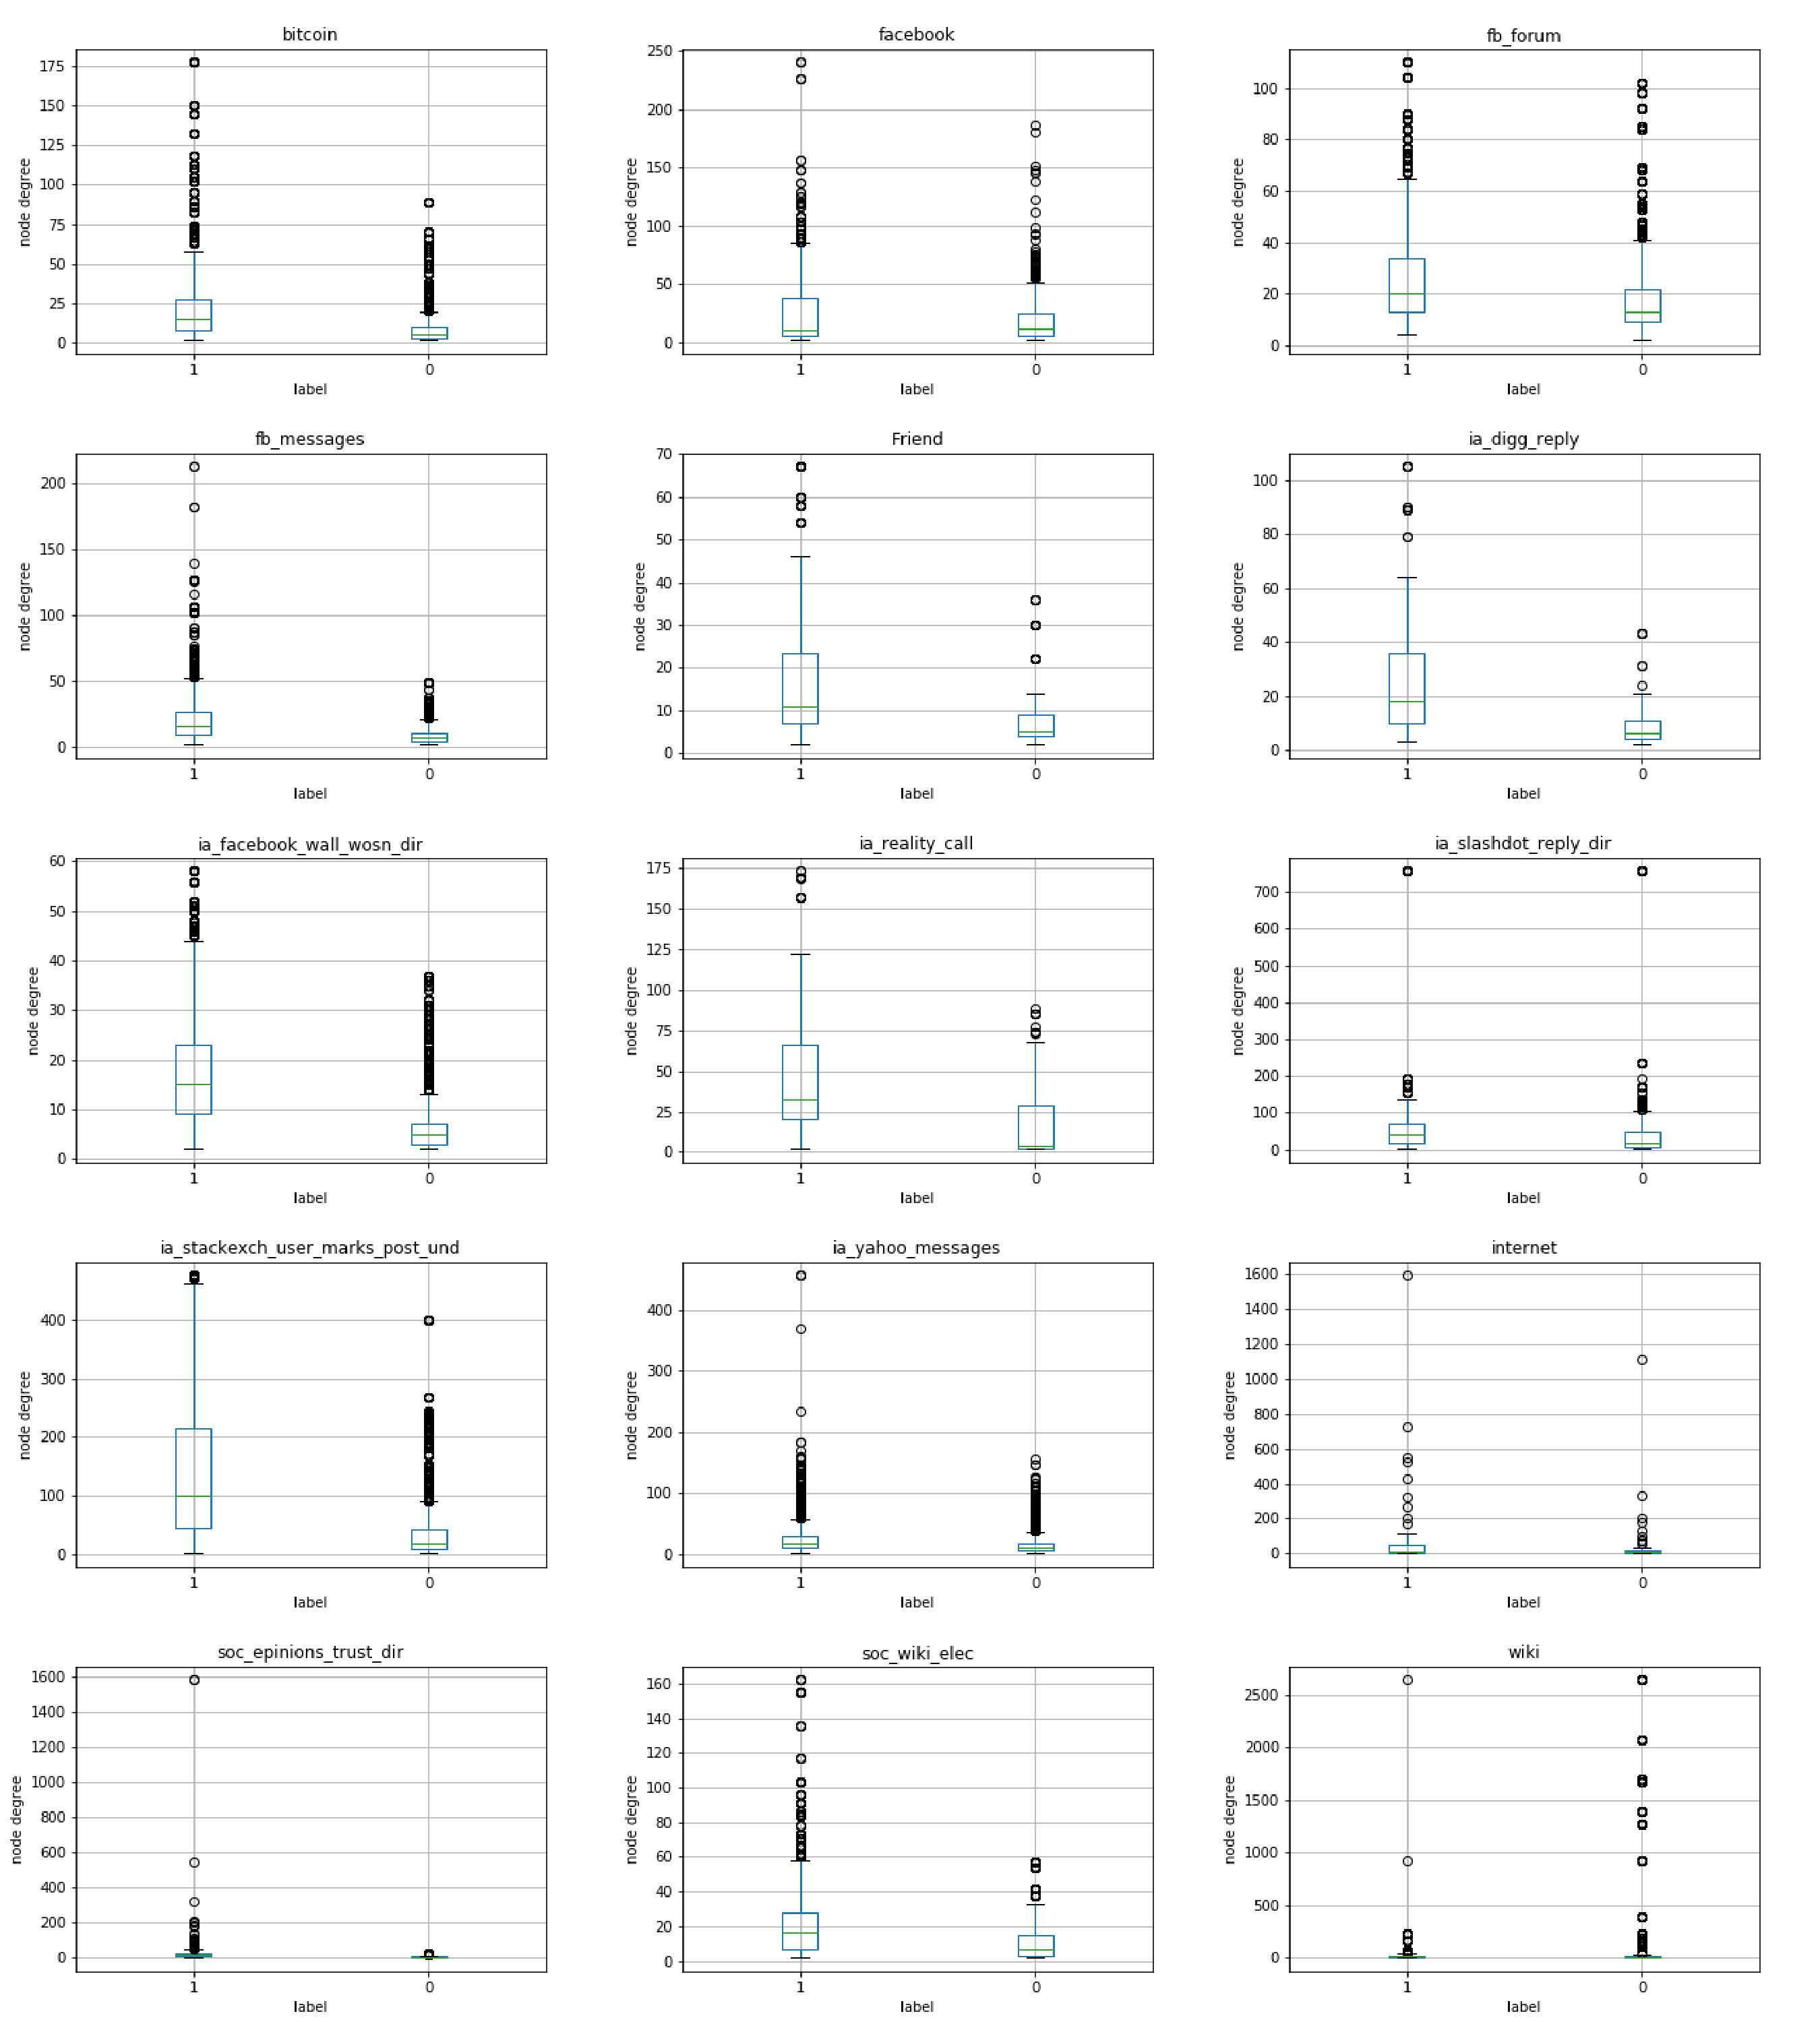
\includegraphics[width=.9\textwidth]{./figure/alldata-DG.pdf}
	\caption{15个数据集的节点度的分位图}
	\label{fig.3.4}
\end{figure}

\begin{figure}[!htbp]
	\setlength{\abovecaptionskip}{0pt} 
	\setlength{\belowcaptionskip}{10pt} 
	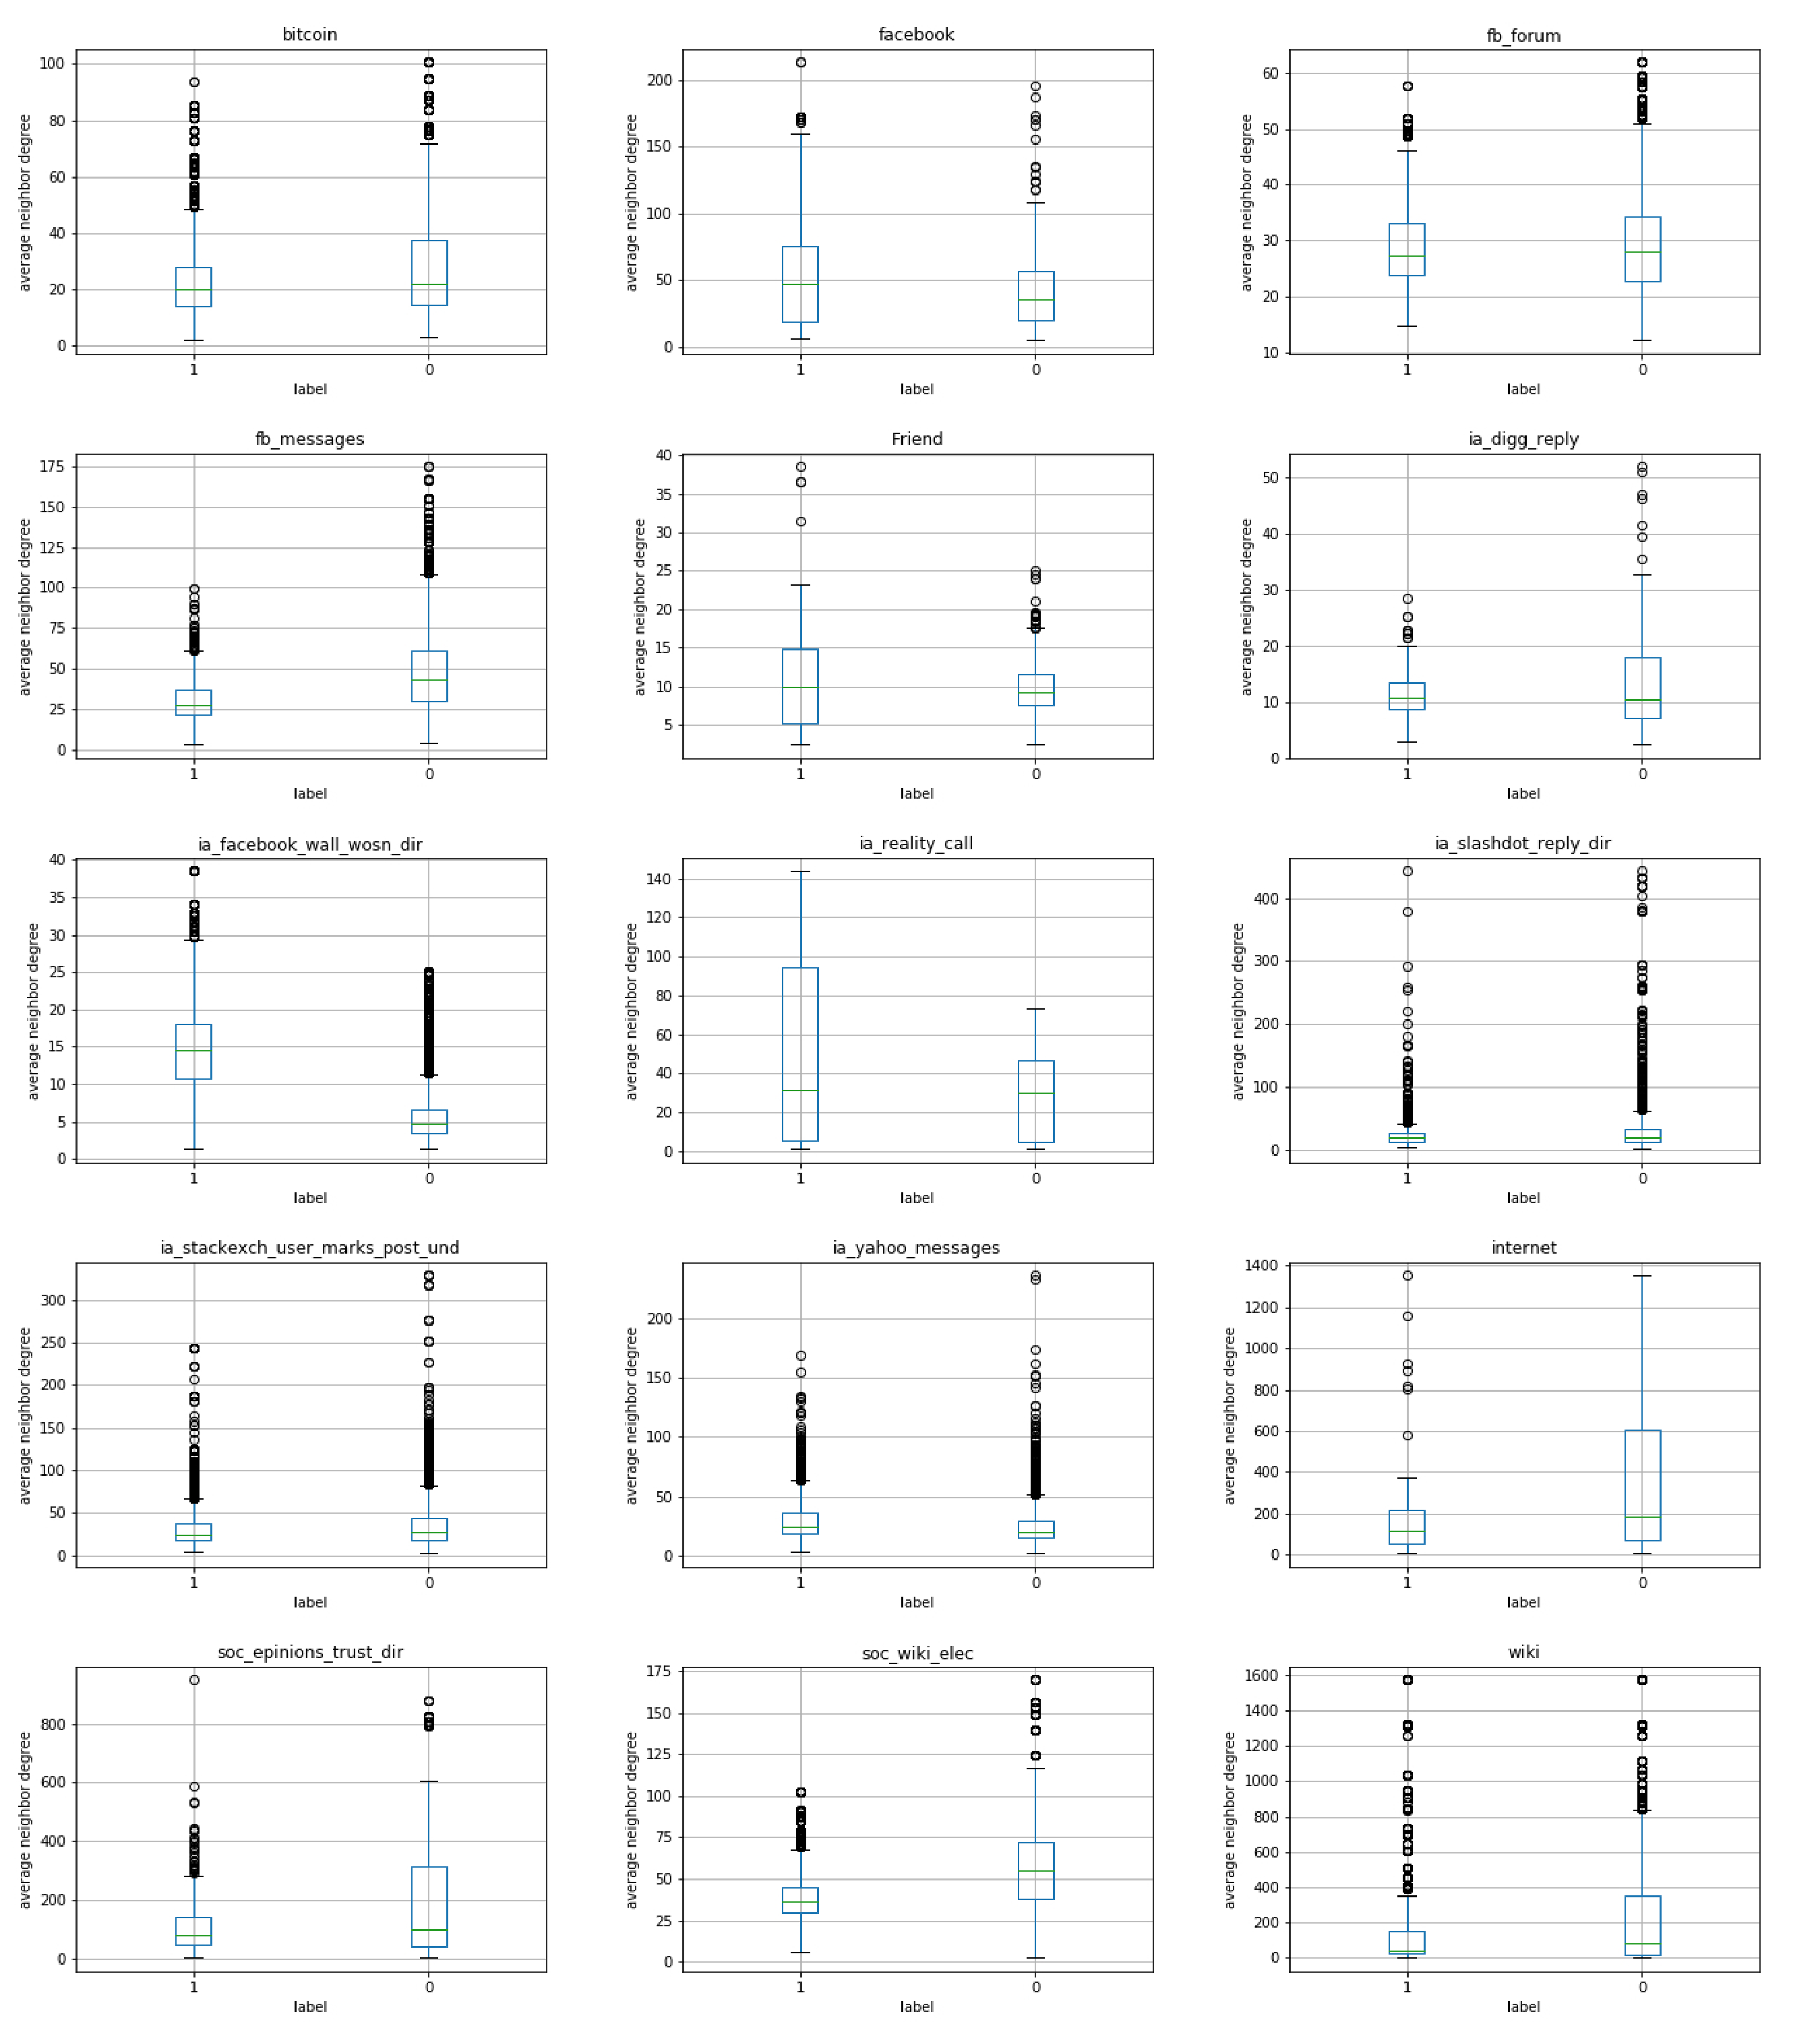
\includegraphics[width=.9\textwidth]{./figure/alldata-aND.pdf}
	\caption{15个数据集的节点的平均邻居度的分位图}
	\label{fig.3.5}
\end{figure}


\subsection{验证}

为了验证结论\textbf{节点的度及节点的平均邻居度影响节点的社团转移},本文在论文引用网络DBLP中支撑结论的案例。如图\ref{fig.3.6}所示,图中节点代表论文作者,而节点大小代表节点的度的大小。不同颜色代表节点所属社团不同,即不同颜色作者的研究兴趣不同,同时节点上的文字代表“平均邻居度-作者名”,例如“4.82-$Shuicheng Yan$”代表作者名为$Shuicheng Yan$的平均邻居度为$4.82$。

其中图\ref{a}\ref{b}展示了平均邻居度给论文作者带来的影响,图\ref{a}与图\ref{b}是相邻时间快照($2005$年和$2006$年)的相同作者的论文发表可视化图。可以看到,$Jun Yan,Zheng Chen$和$Ning Liu$ 都具有较高的平均邻居度$9.33$,受他们共同的具有较高节点度的邻居$Shuicheng Yan$的影响,在$2006$年,他们转移了原有的研究兴趣领域,在\texttt{TKDE}上与$Shuicheng Yan$合作发表了与$Shuicheng Yan$相同研究兴趣的论文\footnote{Yan, Jun, et al. "Effective and efficient dimensionality reduction for large-scale and streaming data preprocessing." IEEE transactions on Knowledge and Data Engineering 18.3 (2006): 320-333.}。

而图\ref{c}\ref{d}则展示了节点度对论文作者带来的影响,图\ref{c}和图\ref{d}也是相邻时间快照($2005$年和$2006$年)相同作者的论文发表可视化图。如图所示,$Marc Pollefey$所属的节点具有较大的直径,即其节点度较大,这代表着他的朋友较多,而由图\ref{c}可以看出,他的绝大部分朋友都与他所在的研究兴趣领域不同。受其朋友影响,他在$2006$年改变了其研究兴趣领域。更详细的说,他与他的合作者$Jan-Michael Frahm$在$2006$年在\texttt{EDGE}共同发表了一篇论文 \footnote{Sinha, Sudipta N., et al. "GPU-based video feature tracking and matching." EDGE, workshop on edge computing using new commodity architectures. Vol. 278. 2006.}。从图中的两个较小的节点$Roland Memisevic$和$Christopher Zech$也能看出平均邻居度的影响,这二人都具有较高的平均邻居度$8.33$,而受到两人共同的朋友$Marc Pollefeys$的影响,他们也在$2006$年改变了研究兴趣领域。

\begin{figure}[!htbp]
	\centering
	\subfigure[]{
	\begin{minipage}[t]{0.48\textwidth}
		\centering
		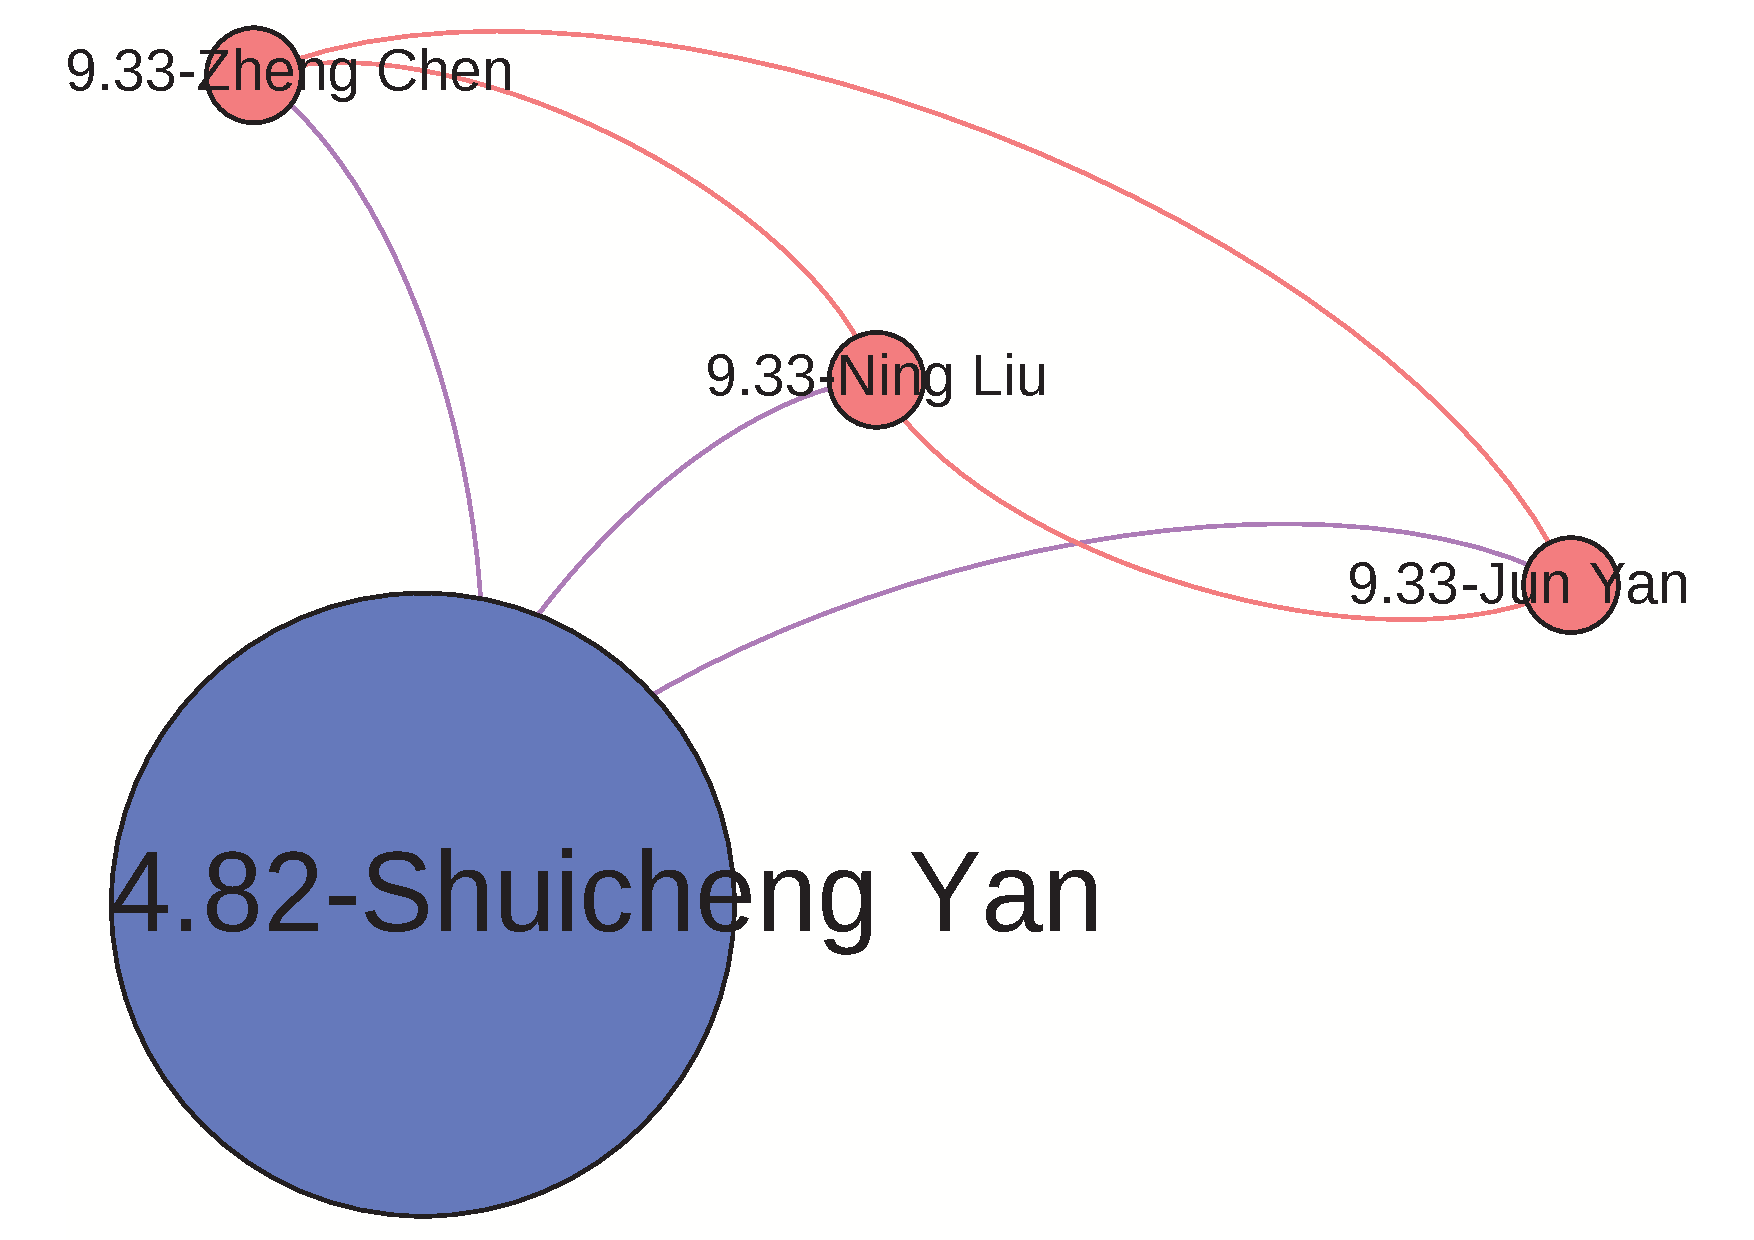
\includegraphics[width=4cm]{./figure/ca0.pdf}
		\label{a}
	\end{minipage}}
	\subfigure[]{
	\begin{minipage}[t]{0.48\textwidth}
		\centering
		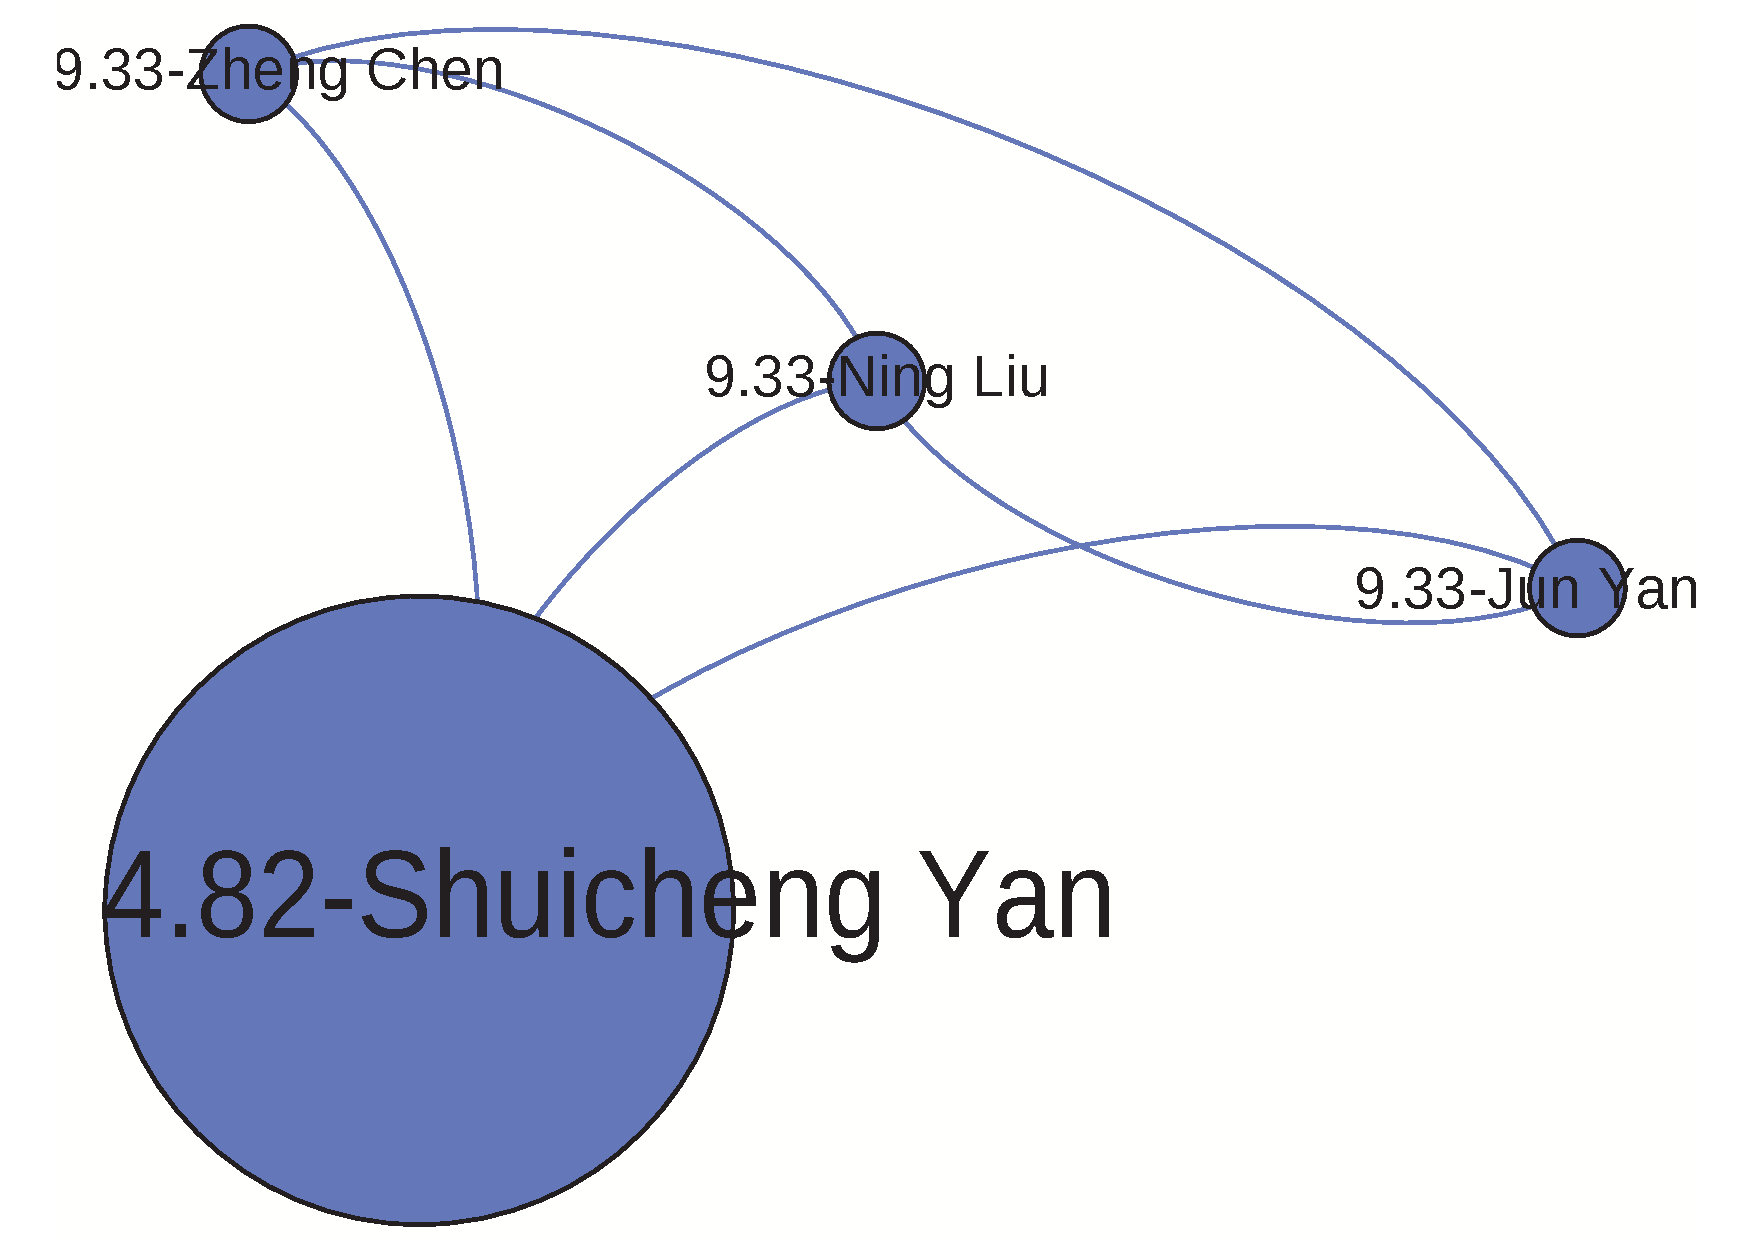
\includegraphics[width=4cm]{./figure/ca1.pdf}
		\label{b}
	\end{minipage}}
	\subfigure[]{
	\begin{minipage}[t]{0.48\textwidth}
		\centering
		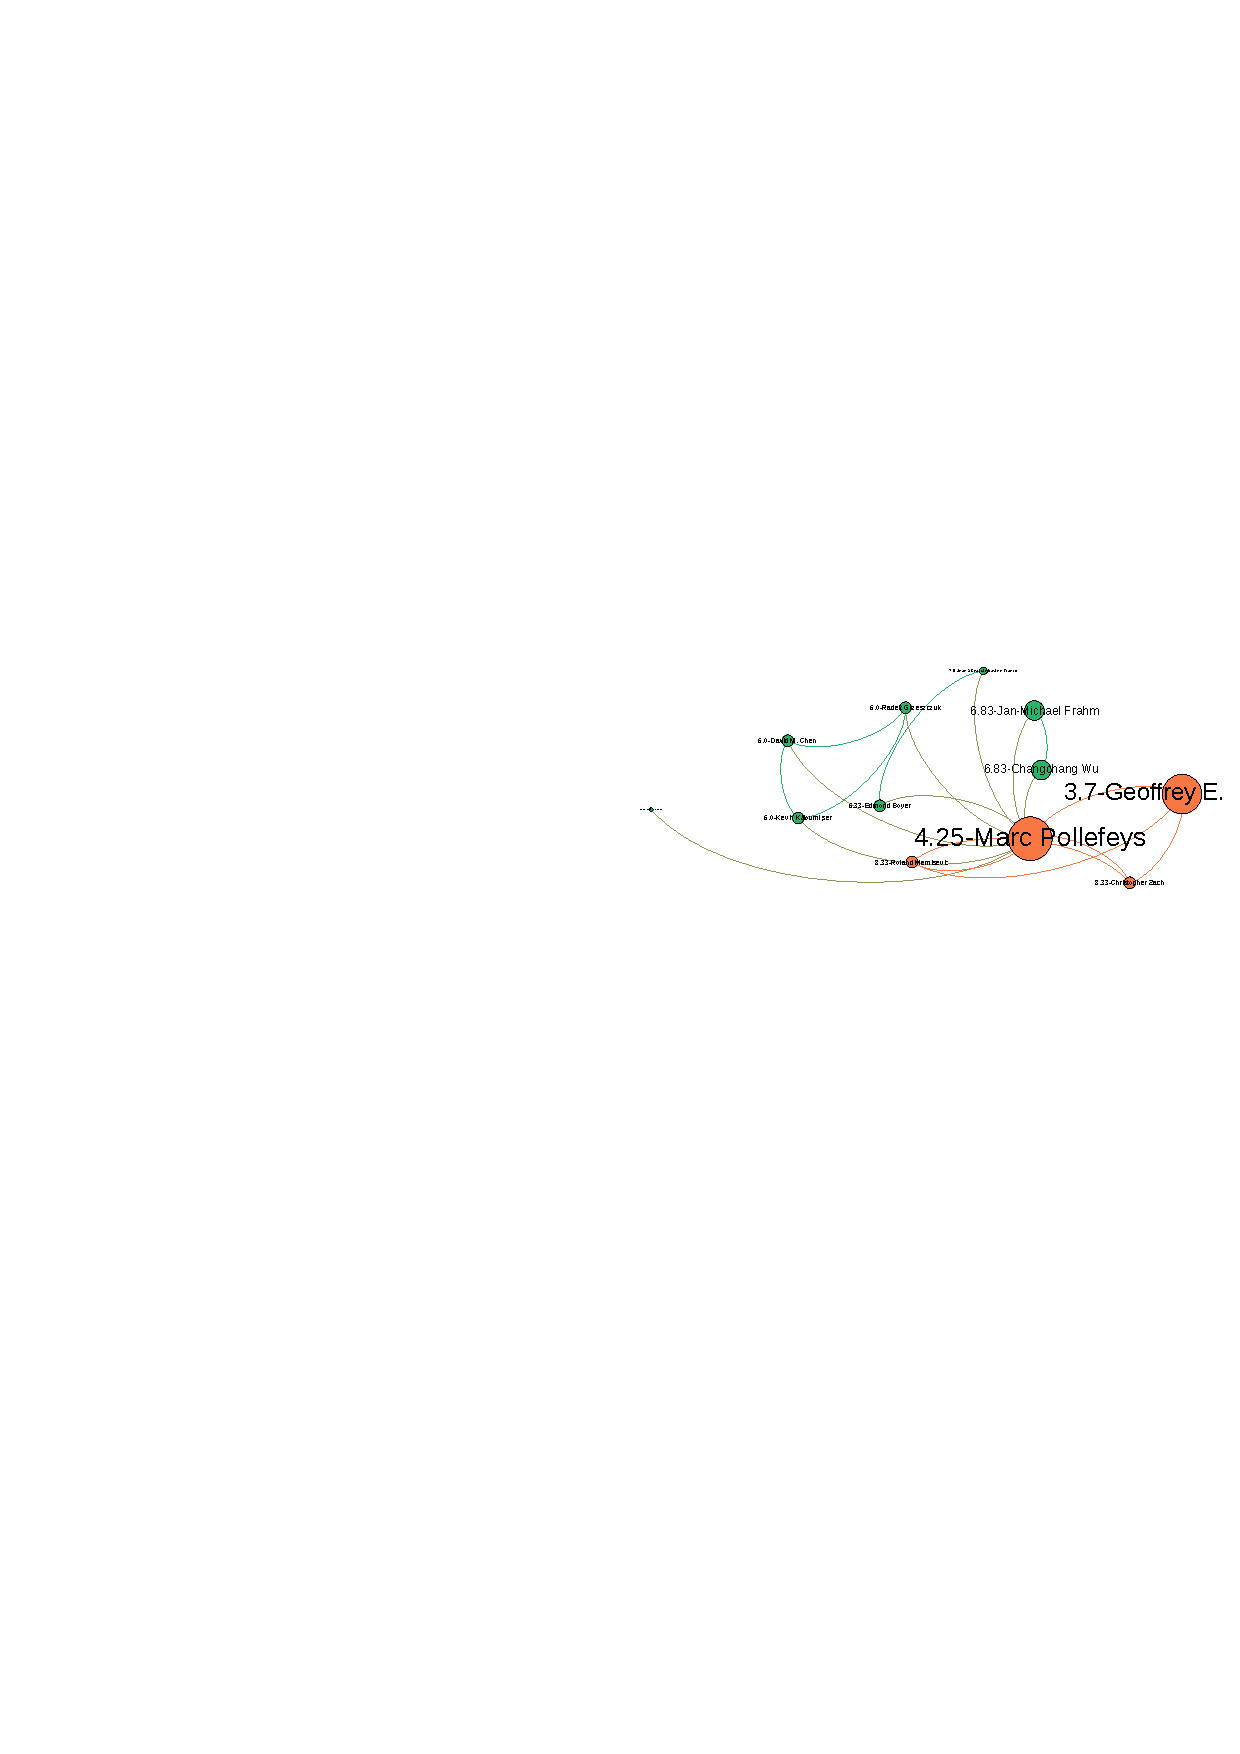
\includegraphics[width=6cm]{./figure/case0.pdf}
		\label{c}
	\end{minipage}}
	\subfigure[]{
	\begin{minipage}[t]{0.48\textwidth}
		\centering
		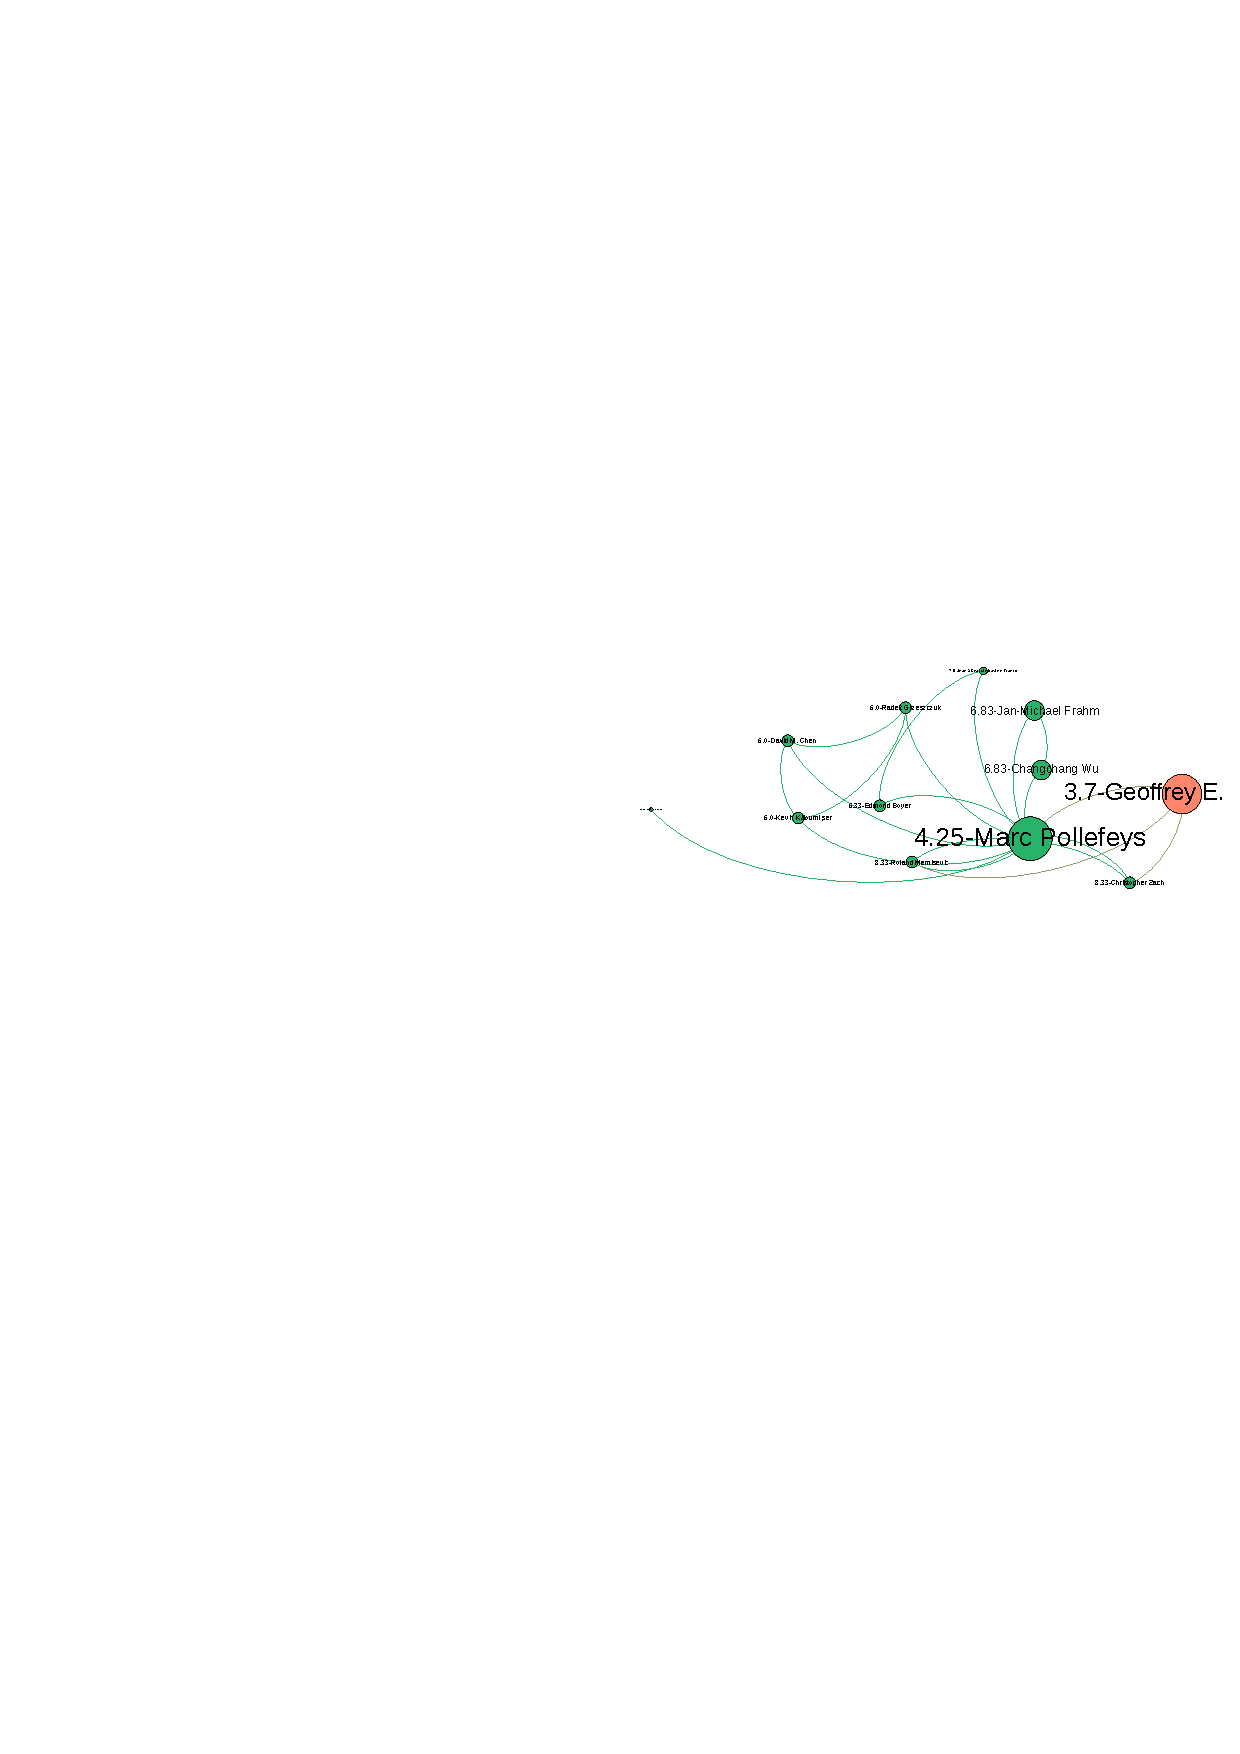
\includegraphics[width=6cm]{./figure/case1.pdf}
		\label{d}
	\end{minipage}}
	\caption{基于DBLP数据的验证案例}
	\label{fig.3.6}
\end{figure}

\section{本章小结}

通过将节点的结构属性视为分类特征,并将节点是否发生社团转移视为分类标签,本章利用决策树对其进行二分类,并分析了节点特征在分类中的重要性。最终得出结论:节点的度以及节点的平均邻居度对节点的社团转移影响最大且最为广泛。同时本章还在DBLP中找到了支撑结论的样例。下一章将会介绍受本章启发并改进自DSBM的社团检测生成模型HB-DSBM。


























